\section{Liste des scenarii SAP}

\subsection{Gestion des contrats clients}

\begin{figure}[H]
    \label{fig-gestion-contrats-client}
    \noindent\makebox[\textwidth]{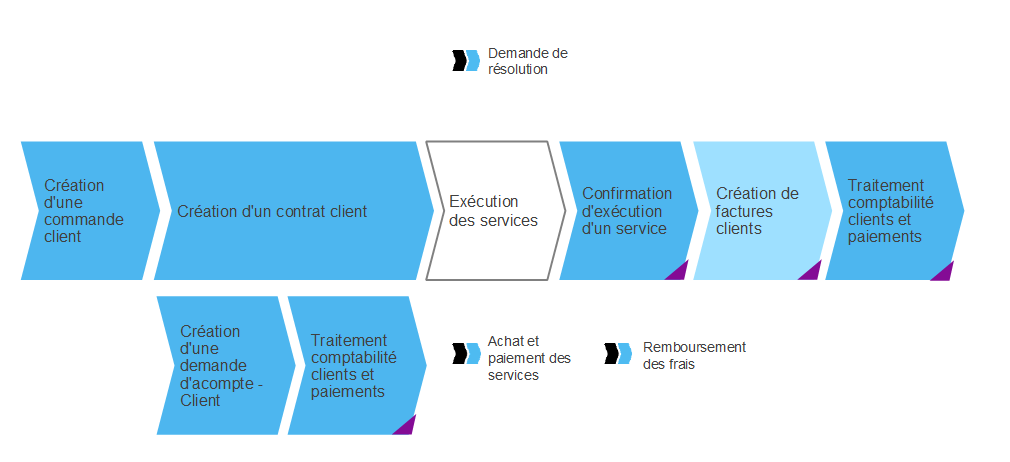
\includegraphics[width=15cm]{figures/gestion_contrats_client.png}}
    \caption{Gestion des contrats clients}
\end{figure}

Le scénario gestion des contrats clients permet de créer et de gérer les contrats relatifs aux services et se décline en 6 axes principaux : \\

\begin{enumerate}
\item Création d’une commande client \\
Ce processus sert à créer une commande, en réponse à une commande client de produits ou services. Un contrat est automatiquement généré pour ce poste à l’aide d’un modèle de contrat. La commande client peut éventuellement être approuvée. \\

\item Création d’un contrat client \\
Ce processus permet de créer un contrat portant sur des services, des frais ou des droits. Pour cela, il est possible d’utiliser un modèle de contrat dont les données sont copiés dans le nouveau contrat.\\

\item Exécution des services \\
Ce processus permet à l’ingénieur services, après validation de l’ordre pour exécution et une fois les préparatifs effectués, de se rendre chez le client pour exécuter le service demandé, ou d’exécuter le service à distance ou sur un site de réparation. \\

\item Confirmation d'exécution d’un service \\
Ce processus permet à l’ingénieur service d’achever son travail, après l’exécution d’un service, en créant une confirmation de service pour déclarer les temps réels. La confirmation de service sert aussi à enregistrer des informations supplémentaires sur le travail exécuté. \\

Une fois le document de confirmation de service validé, la facturation client est déclenchée automatiquement et les informations nécessaires sont transmises à la comptabilité financière. \\

\item Création des factures clients \\
Dans ce processus, les demandes de factures sont créées automatiquement après la prestation de services. Ces demandes doivent être transférés vers une facture, qui est envoyée au client et transmise à la gestion des flux de trésorerie. \\

\item Traitement des paiements initiés en externe par virement reçu \\
Ce processus permet le paiement par virement bancaire des factures clients dont le paiement est initié en externe.
\end{enumerate}

\subsection{Service et réparation}

\begin{figure}[H]
    \label{fig-service-reparation}
    \noindent\makebox[\textwidth]{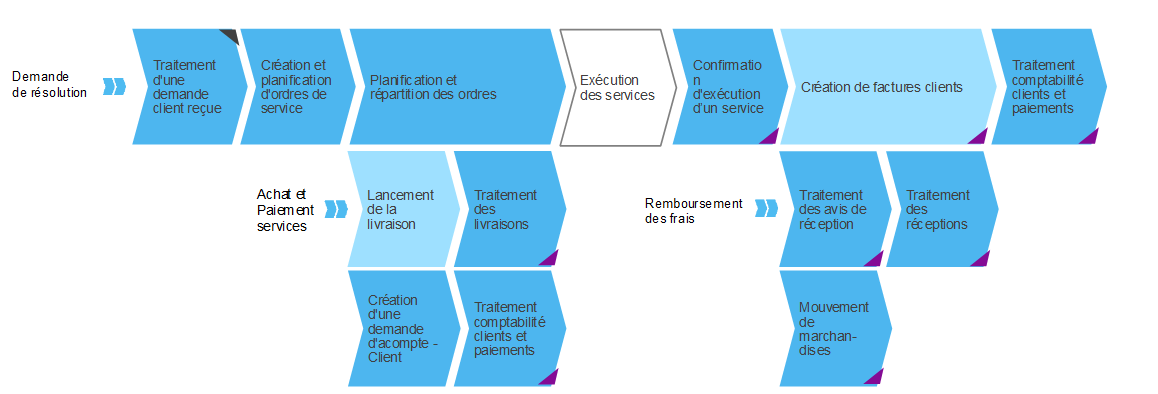
\includegraphics[width=15cm]{figures/service_reparation.png}}
    \caption{Service et réparation}
\end{figure}

Le scénario service et réparation permet d’assurer des services de réparation et de maintenance sur site. Il se décline en 7 axes principaux. Nous ne détaillons que les 3 premiers processus, les 4 derniers étant déjà présents dans le scénario Gestion des contrats clients. \\

\begin{enumerate}
\item Traitement d’une demande client reçue \\
Ce processus permet de gérer la réception de demandes via différents canaux d’entrée, comme le téléphone ou l’e-mail. \\

\item Création et planification d’ordres de service \\
Ce processus permet au service client de créer un ordre de service quand un client demande la réparation ou la maintenance d’un produit. \\

\item Planification et répartition des ordres \\
Ce processus permet aux salariés des services d’affecter un ordre, manuellement ou automatiquement, à l’ingénieur service et à l’équipe d’exécution. Il peut ensuite planifier l’intervention de l’ingénieur service. \\

\item Autres axes \\
Le scénario SAP comprend aussi les axes d’exécution des services, de confirmation d’exécution d’un service, de la création des factures clients et du traitement des paiements initiés en externe par virement reçu. Nous ne détaillons cependant pas plus ces axes ici car nous les avons déjà évoqués précédemment.
\end{enumerate}

\subsection{Gestion des commandes}

\begin{figure}[H]
    \label{fig-gestion-commandes}
    \noindent\makebox[\textwidth]{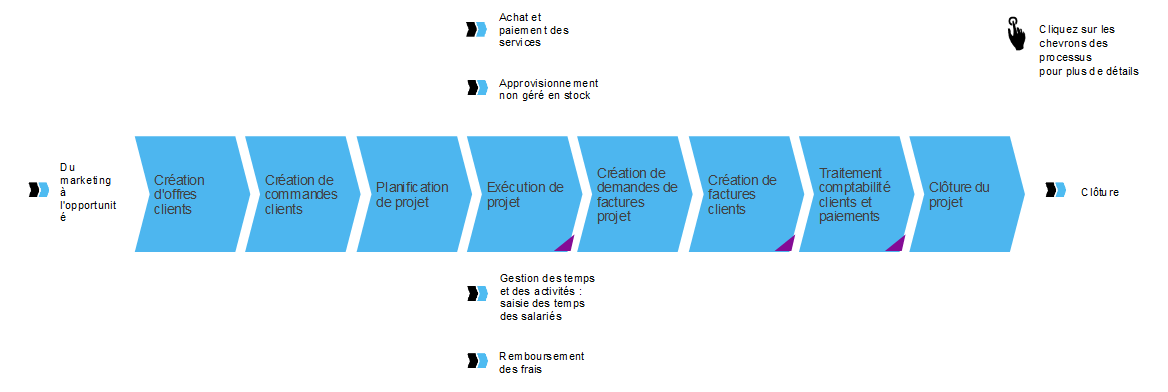
\includegraphics[width=15cm]{figures/gestion_commandes.png}}
    \caption{Gestion des commandes (services et produits basés sur le projet)}
\end{figure}

Le scénario Gestion des commandes (services et produits basés sur le projet) permet de gérer de bout en bout la vente aux clients de ce type de services et produits. Grâce à l'intégration des offres et commandes clients à la gestion de projets, il est possible de créer des factures clients conformes aux temps et frais saisis pour un projet client. Les factures peuvent être établies sur une base réelle, forfaitaire ou mixte. Une fois la facture client émise, les paiements client peuvent faire l'objet d'un suivi. 
Ce scénario prend également en charge l'analyse de la rentabilité du projet sur la base de ses coûts et produits. \\

\begin{enumerate}
\item Création d’offres clients \\
Le processus de gestion Création d'offres clients sert à créer une offre client à durée et prix fixes, en réponse à une demande client d'offre de  produits ou services. L'offre client peut aussi être générée à partir d'une opportunité ou d'un intérêt potentiel. \\

\item Création de commandes clients \\
Le processus de gestion Création de commandes clients sert à créer une commande à durée et prix fixes, en réponse à une commande client de produits ou services. Il est possible de créer la commande en référence à une offre et reprendre toutes les conditions de l'offre dans la commande ou d’en saisir les données requises (compte, produits ou services et date
demandée), ainsi que des informations client complémentaires. \\

\item Planification de projet \\
Le processus de gestion Planification de projet facilite la création, planification et structuration du projet, la configuration de l'équipe et sa dotation en ressources. \\

\item Exécution de projet \\
Le processus de gestion Exécution de projet inclut la validation du projet avec la création de l'état de référence, l'affinement du plan de projet, la constitution de l'équipe et l'affectation de personnel.
\end{enumerate}


